\section{Devices and Setup}
In this section we give a short overview over the setup, introducing the used devices and sources of radiation. We
further specify the procedure for the measurements. 

\subsection{Sources of radiation}
\label{sec:sources}
We conduct the experiment for the case of $\gamma$-rays, using two different sources. The first sample is a 
\textit{$^{22}$Na}  sample exclusively used for calibration and setting of delays. The unstable isotope decays by 
$\beta^+$ decay with a life time of 2.6 a. Another observed decay is via K electron capture, being ten times less likely. 
Both decays can be described as
\begin{align}
_{11}^{22}\text{Na}        \quad &\rightarrow \quad _{10}^{22}\text{Ne}^* + e^+ + \nu_e	\qquad \text{($\beta^+$ decay)} \\
_{11}^{22}\text{Na} + e^-  \quad &\rightarrow \quad _{10}^{22}\text{Ne}^* + \nu_e  \qquad \text{(K electron capture)}
    \label{eq:22na_decay}
\end{align}
The excited $^{22}$Ne has a life time of 5 ps and returns to its ground state emitting a photon with an energy of 
1275~keV.\cite{lnhb} The $^{22}$Na is very useful for the setting of the delays because two photons originating from the 
annihilation of the $e^+$ are highly correlated in direction ($180^\circ$).\cite{ver}

The second source is a \textit{$^{137}$Cs} sample which decays to with a life time of 30 emitting electron 
($\beta^-$ decay):
\begin{equation}
_{55}^{137}\text{Cs} \quad \rightarrow \quad _{56}^{137}\text{Ba}^* + e^- + \bar{\nu}_e \qquad \text{($\beta^+$ decay)}
    \label{eq:137cs_decay}
\end{equation}
The excited Barium decays with a life time of 2.5 min under the emission of a 661.7 keV photon.\cite{lnhb} 
These photons will be the source of radiation for the Compton scattering in our experiment.

\subsection{Scintillators}
\label{sec:scinti}
We use two different scintillators for detecting the scattered electrons and photons, respectively. Scintillators work by 
emitting light when exposed to ionizing radiation. The light can be amplified by a photo multiplier and transformed to an 
electric signal. 
The \textit{organic scintillator} is used for the detection of electrons. It is a PVC scintillator and further the site of 
scattering, i.~e. electrons of the polymers are scattered and recorded without leaving the scintillator. Because the 
absorption coefficient due to the photo effect is very small, most scattered photons leave the scintillator. 
The \textit{inorganic scintillator} on the other hand detects the scattered photons. The latter produce electron gaps that 
emit light when falling back to the ground state. The applied scintillator is a NaI(Tl) crystal. It's absorption coefficient 
for the photo effect is much larger for photons between 0.5 and 1 MeV. Absorption coefficients for all three effects --
photo and Compton effect as well as pair production -- can be seen in figure~\ref{fig:nai_absorption}. 

\begin{figure}[htpb]
    \centering
    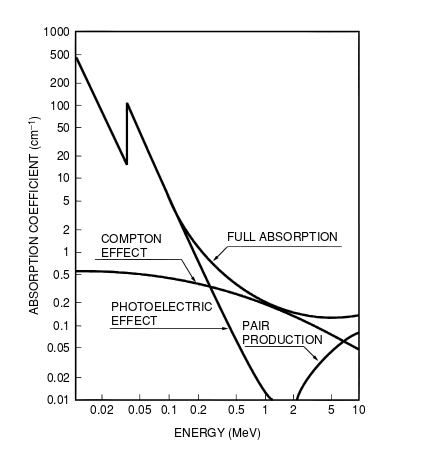
\includegraphics[width=0.5\linewidth]{figures/nai_absorption}
    \caption{
        Absorption coefficient of NaI(Tl) scintillator for $\gamma$-rays. Photons in this experiment have energies 
        between 0.1 and 1 MeV. Taken from \cite{hamamatsu}. 
        }
    \label{fig:nai_absorption}
\end{figure}




\subsection{Experimental Setup}
\label{sec:label}
The setup of the experiment contains the source of radiation, both scintillators and a delayed coincidence circuit for 
signal processing. The analogue signals are finally transformed to digital data by a multi channel analyzer (MCA) and 
saved in histograms. The setup containing the full coincidence circuit is shown in figure~\ref{fig:setup}. The 
preamplifier (PA) and main amplifier (MA) enlarge the signal of the photo multiplier (PM) driven by a high voltage (HV).
The MA's front out signal is sent to a timing single channel analyzer (TSCA) which produces a normed logical signal. 
The normed peaks of both TSCA's are fed to a coincidence, yielding in turn a normed logic signal when both signals 
coincide for a predefined time scale.
The rear out signal of the MA is delayed and put through a logic gate which receives the signal of the coincidence, such 
that both coincidence and peak intensity can be measured by the MCA. The Hex Scale is used during the setup only, namely
for determining the correct delays.

\begin{figure}[htpb]
    \centering
    \includegraphics[width=0.8\linewidth]{figures/setup}
    \caption{
        Scheme of the full setup of the experiment. All abbreviations are explained in the text.
        }
    \label{fig:setup}
\end{figure}


\subsection{Measurement Procedure}
\label{sec:procedure}
The experiment consists to a large part of a careful calibration and setting of the correct setup, while the actual 
central measurements are a rather automatized procedure. We start of by a calibration of the two scintillators. 
This is done with the full setup except for the coincidence and logic gates. We take full spectra of both samples for 
both scintillators in order to fit the linear correspondence between channels and actual energies. For the NaI 
scintillator, we know both the photo peaks at of the samples as well as Compton edges:
\begin{itemize}
    \item for the $^{137}$Cs sample: a Compton edge at 447 keV and an escape peak at 183 keV;
    \item for the $^{22}$Na sample: Compton edges at 341 keV and 1064 keV corresponding to photo peaks at 511 keV and 
        1064 keV, respectively.
\end{itemize}
For the PVC scintillator, the situation is worse since photons are not detected to a considerable amount. 
Only the Compton edges are visible, yielding only the three points at 447, 341 and 1064 keV. 
After measuring these spectra, we chose windows on the TSCAs in order to reduce background, most notably of very low 
energies. We then set up the coincidence section by maximizing the rate measured with the Hex Scale for 
coincidences. This is done with the $^{22}$Na sample in between the two scintillators. Since the Hex Scale only accepts 
normed negative pulses, we have to transform the positive square put out by the coincidence device using a TSCA. 
An oscilloscope is further used to observe the overlay of the signals. Once this step is complete, we use the oscilloscope 
in order to set the delay of the linear signal that is to be measured such that its maximum coincides with the center 
of the logical window generate with the same signal. This is done since the MCA uses the amplitude of a signal in order 
to assign a channel. The step has to be repeated before each measurement since delays for signals of either scintillator 
are not necessarily the same. 

When these preparations are complete, we start measuring the spectra of PVC and NaI scintillator in coincidence for 
angles from 0 to 120$^\circ$ in steps of $15^\circ$ using the $^{137}$Cs as a source. The measurement time for this 
part is set to 3600 s. In order to interpret 
these measurements correctly, we have to take measurements on the background (i.~e. without the source) as well as on the 
random coincidence with the sample. This is done by setting one of the delays of the TSCAs to a value far from the chosen 
one for coincidence. Signals will thus only overlap randomly. Finally, we have to measure the total incident radiation 
in the solid angle covered by the NaI scintillator. This is done by removing the PVC scintillator entirely.  


